\documentclass[a4paper,12pt]{article}
\parindent 0pt
\parskip 1mm
\usepackage[dvips]{epsfig}

\begin{document}

\begin{center}
{\Large\bf CN 510 - Principles and Methods of Cognitive and Neural Modelling}

\bigskip

{\large\bf Assignment \# 1}
\smallskip

{\large\bf John Joseph}
\end{center}

We are given the following non-homogeneous differential equation

\begin{equation}
\frac{dx}{dt} + Ax = I
\end{equation}

\bigskip
{\bf Analytic Solution}
\bigskip

The solution of course exists in two parts: homogeneous, and particlar. The homogenous solution can be found as follows:

\begin{equation}
\frac{dx_h}{dt} + Ax_h = 0
\end{equation}
\begin{equation}
\frac{dx_h}{dt} = -Ax_h
\end{equation}
\begin{equation}
x_h(t) = Ce^{-At}
\end{equation}

Now that we have the homogeneous solution, let us solve for the particular solution. 

\begin{equation}
\frac{dx_p}{dt} + Ax_p = I
\end{equation}
\begin{equation}
x_p(t) = mt+b
\end{equation}
\begin{equation}
\frac{dx_p}{dt} + Ax_p = m + A(mt+b) = I
\end{equation}
\begin{equation}
m = 0
\end{equation}
\begin{equation}
b = \frac{I}{A}
\end{equation}
\begin{equation}
x_p(t) = \frac{I}{A}
\end{equation}

Thus, the solution to this differential equation is

\begin{equation}
x(t) = Ce^{-At} + \frac{I}{A}
\end{equation}

As you can see, this equation depends on three initial parameters: $x_0$, $I$, and $A$. These will be required not only to fully solve and plot the analyitic solution; we also require these boundary conditions be set in order to use numerical methods in calculating the solution.

\bigskip
{\bf Analytic Results}
\bigskip 

Here you can see the results to the analytical solution we have just derived. These plots each show to outcomes to the solution based on different initial conditions, set by $x_o$, $I$ and $A$.

\bigskip
{\bf Analysis}
\bigskip 

Note that the system described by the equation 

\begin{equation}
x(t) = Ce^{-At} + \frac{I}{A}
\end{equation}

actually converges to an equilibrium state as our variable representing time, $t$, approaches larger values. We can see the exponential portion of the term contains a negative sign in its power, so as $t$ gets larger and larger the exponential term starts to vanish. Once this term has grown sufficiently small, the outcome of the above equation will be extremely close to the constant term $\frac{I}{A}$. 

From the plots above we can see that our results to approach these equilibrium states, states which again depend on the initial conditions. For example, when $x_0=0$, $I=5$ and $A=1$, we see the solution eventually converges on $x=5$. You can see this trend in all four lines , and as $t->5$ the results become nearly identical to the expected value. 

\begin{figure}[h!]
\begin{center}
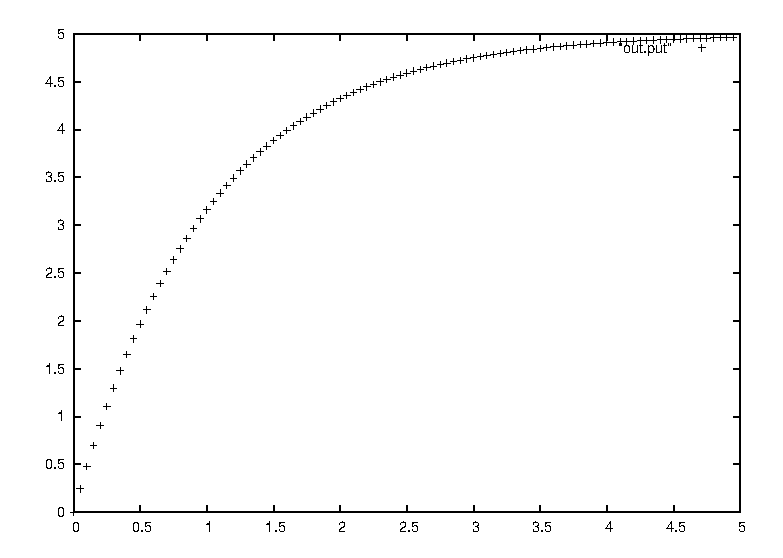
\epsfig{file=graph1,width=11cm,height=8cm}
\end{center}
\caption{\label{pict1} The above equation solved from t=0 to t=5. }
\end{figure}

 

\begin{figure}[h!]
\begin{center}
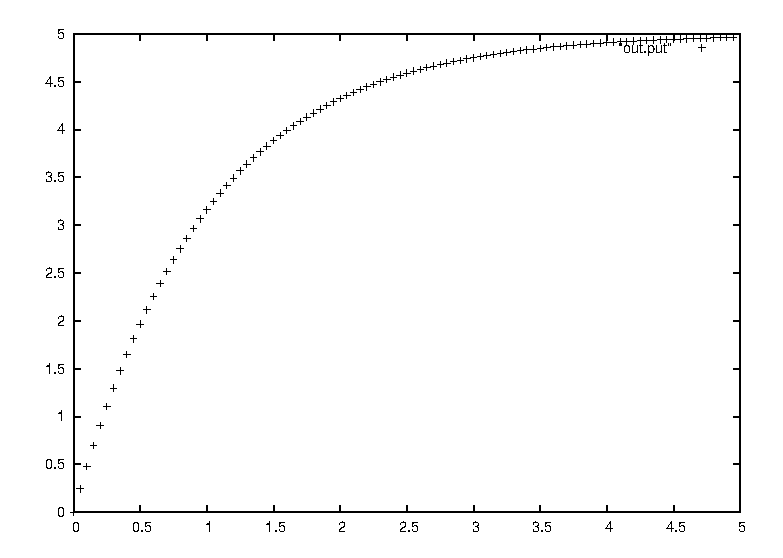
\epsfig{file=graph1,width=11cm,height=8cm}
\end{center}
\caption{\label{pict1} The above equation solved from t=0 to t=5. }
\end{figure}

\end{document}
